Features expected from the application will be written down in this chapter.
All information needed was gathered in an interview with the thesis supervisor, an experienced \etl{} user.
\section{Requirements}
In this section, granular requirements are gathered and described.

\subsection*{F-1.1: Settings screen}
Application must have a separate screen for settings.
\subsection*{F-2.1: View server instance}
List of server instances will be visible from settings screen.
\subsection*{F-2.2: Add server instance}
User must be able to add server instance.
\subsection*{F-2.3: Edit server instance}
User must be able to edit already added server instance.
\subsection*{F-2.4: Delete server instance}
User must be able to delete already added server instance. It will be possible to undo the action.
\subsection*{F-2.5: Deactivate server instance}
User can deactivate server instance in settings instead of deleting it, so it is possible to activate it again later easily. App will not communicate with deactivated server instances.
\subsection*{F-2.6: Ping server}
\label{subsec:ping}
User can test if the server address is correct.
\subsection*{F-2.7: Load server instance info from QR code}
\label{subsec:qrcode}
User can load server instance URL from QR code.
\subsection*{F-3.1: Notification after pipeline execution finish}
\label{subsec:notifications}
Application shell create a notification on pipeline execution finish.
\subsection*{F-3.2: Notifications in settings}
It will be possible to toggle notifications in settings.
\subsection*{F-4.1: Pipeline list screen}
Application must have a separate screen for working with pipelines. Which pipelines will be visible there depends on F-4.8.
\subsection*{F-4.2: View pipelines}
List of pipelines will be visible from pipeline list screen. Which pipelines will be visible depends on F-4.8.
\subsection*{F-4.3: Edit pipeline screen}
\label{subsec:editpipelinescreen}
Application must have a screen for editing pipelines.
\subsection*{F-4.4: Create pipelines}
User must be able to start an empty edit pipeline screen (F-4.3) from the pipeline list screen (F-4.1).
\subsection*{F-4.5: Edit existing pipelines}
User must be able to edit selected pipeline by starting the edit pipeline screen (F-4.3) with the selected pipeline loaded.
\subsection*{F-4.6: Delete pipelines}
User must be able to delete a pipeline of his choice.
\subsection*{F-4.7: Execute pipeline}
User must be able to execute selected pipeline.
\subsection*{F-4.8: Source for visible pipelines}
User must be able to choose, if he wants to see pipelines from all instances, or just a specific one.
\subsection*{F-5.1: Execution history screen}
Application must have a separate screen for execution history. History of which server instance will be visible depends on F-5.5
\subsection*{F-5.2: View execution history}
List of executions will be visible from the execution history screen. History of which server instance will be visible depends on F-5.5
\subsection*{F-5.3: Delete execution from history}
User must be able to delete a specific execution from the execution history. It will be possible to undo the action.
\subsection*{F-5.4: Re-execute pipelines from history}
There must be an option to re-execute pipeline from the execution history screen. This action will also make a new record in execution history.
\subsection*{F-5.5: Source of visible history}
User must be able to choose, if he wants to see history of all instances, or just a specific one.
\subsection*{F-6.1: Night mode}
User can have an option in settings to use light or dark theme, or use system default theme (Android 10 and newer).












\section{Use cases and scenarios}
In this section, use cases, representing reasons why users want to use our application, will be described and complemented by scenarios, describing how to achieve the goals of those use cases.
This section is supplemented by a diagram concluding use cases.
See \autoref{fig:uc}


\subsection*{UC-1: Get overview of executions in particular server instance}
Enables user to see what pipelines were executed in chronological order from specific server instance.

\begin{itemize}
\item \textbf{SC-1.1: Get overview of executions in particular server instance}
User opens execution history screen (F-5.1, F-5.2) and selects what server instance's executions he wants to see (F-5.5).

\end{itemize}

\subsection*{UC-2: Execute specific pipeline}
Enables user to execute pipeline of his choice from specific server instance.

\begin{itemize}
\item \textbf{SC-2.1: Execute specific pipeline}
User opens pipeline list screen (F-4.1, F-4.2). He then finds the desired pipeline and executes it (F-4.7). Optional: After opening the pipeline screen, user can filter pipelines by the server instance (F-4.8).

\end{itemize}

\subsection*{UC-3: Manage registered server instances}
Enables user to register server instance in the application. Application will check, if IP is already registered or if name of the new server instance is already in use, in order to warn user about duplication or name collision that could cause chaos. It also enables user to change IP address of already registered server instance due to type error or network changes. User can also remove registered server instance.

\begin{itemize}
\item \textbf{SC-3.1: Change IP address or name of registered server instance}
User opens settings screen (F-1.1), selects the desired server instance (F-2.1) for editing (F-2.3). He then changes the IP address and saves the changes.

\item \textbf{SC-3.2: Register server instance}
User opens settings screen (F-1.1), tells the application he wants to register new server instance and proceeds to enter server instance's information (F-2.2) and saves it.

\item \textbf{SC-3.3: Delete registered server instance}
User opens settings screen (F-1.1), views registered server instances (F-2.1) and tells the application what server instance he wants to delete. It will be possible to undo the action (F-2.4).

\end{itemize}

\subsection*{UC-4: Manage pipelines}
Enables user to manage pipelines in desired server instance.

\begin{itemize}
\item \textbf{SC-4.1: Create pipeline}
User opens pipeline list screen (F-4.1). Then he tells the application he wants to create a new pipeline (F-4.4). He chooses a server instance to which the pipeline will be saved and the screen for editing pipeline will be launched (F-4.3) and the user can design a new pipeline here. When he is finished, he will save the pipeline.

\item \textbf{SC-4.2: Edit pipeline}
User opens pipeline list screen (F-4.1, F-4.2). He then finds the desired pipeline and tells the application he wants to edit it (F-4.5). The screen for editing pipeline will be launched (F-4.3) with the selected pipeline loaded so the user can make and save changes here. Optional: After opening the pipeline screen, user can filter pipelines by the server instance (F-4.8).

\item \textbf{SC-4.3: Delete pipeline}
User opens pipeline list screen (F-4.1, F-4.2). He then finds the desired pipeline and tells the application he wants to delete it (F-4.6). It will be possible to undo the action. Optional: After opening the pipeline screen, user can filter pipelines by the server instance (F-4.8).

\end{itemize}

\subsection*{UC-5: Re-execute pipeline from history}
Enables user to quickly execute pipeline he see while viewing history.

\begin{itemize}
\item \textbf{SC-5.1: Re-execute pipeline from history}
User opens execution history screen (F-5.1, F-5.2). He finds a pipeline and realizes he wants to execute it now, so he tells that to the application (F-5.4). Optional: After opening the execution history screen, user can select what server instance executions he wants to see (F-5.5).

\end{itemize}

\subsection*{UC-6: Delete history}
Enables user to delete items from history.

\begin{itemize}
\item \textbf{SC-6.1: Delete history}
User opens execution history screen (F-5.1, F-5.2). He finds a record and realizes that he does not want this record in history anymore, so he tells that to the application (F-5.3). Optional: After opening the execution history screen, user can select what server instance executions he wants to see (F-5.5).

\end{itemize}

\subsection*{UC-7: View execution history}
Enables user to view execution history of all the instances at the same time.

\begin{itemize}
\item \textbf{SC-7.1: Get overview of executions}
User opens execution history screen (F-5.1, F-5.2).

\end{itemize}

\subsection*{UC-8: View pipelines}
Enables user to view pipelines from all the server instances.

\begin{itemize}
\item \textbf{SC-8.1: Get overview of pipelines}
User opens pipeline list screen (F-4.1, F-4.2).

\end{itemize}

\subsection*{UC-9: Be notified on execution finish}
User has the option to be notified about execution completion.

\begin{itemize}
\item \textbf{SC-9.1: Be notified}
User executes specific pipeline, just like in SC-2.1. Application will notify user about the execution completion (F-3.1). Notifying will happen only if it is allowed in settings (F-3.2).

\end{itemize}

\begin{figure}\centering
	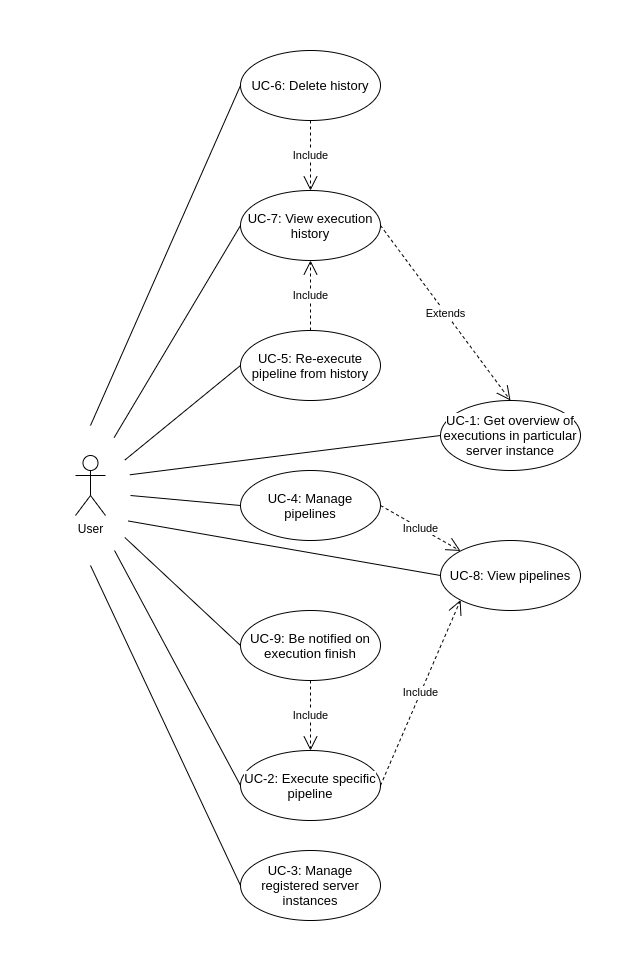
\includegraphics[width=0.9\textwidth]{pics/bc-uc.png}
	\caption[Use cases]{Diagram consisting of use cases}\label{fig:uc}
\end{figure}